\chapter{The Normal Distribution}\index{normal distribution}

Measure the heights of everyone in your grade, and plot them. Most people are near the middle, a few are very
tall or very short, and the picture is a symmetric hill. Test scores, birth weights, and errors in
measurement make the same hill. It is called the \emph{normal distribution}, or the bell curve, and it is the
most important distribution in statistics. In the Continuous Distributions chapter, you learned to describe a
continuous variable with a CDF and a PDF. This chapter applies those tools to the bell curve.

\section{The Normal Distribution}
The Normal distribution, also known as the Gaussian distribution, is a
type of continuous probability distribution for a real-valued random
variable. It is one of the most important probability distributions in
statistics due to its several unique properties and usefulness in many
areas.\index{normal distribution}

\subsection{Defining the Normal Distribution}\index{normal distribution!parameters}

The Normal distribution is defined by its mean ($\mu$) and standard
deviation ($\sigma$). The \index{probability density function}probability density function (pdf) of a
Normal distribution is given by:

\begin{equation*}
f(x|\mu, \sigma^2) = \frac{1}{\sqrt{2\pi\sigma^2}} \exp\left(-\frac{(x-\mu)^2}{2\sigma^2}\right)
\end{equation*}

where:
\begin{itemize}
\item $x$ is a value of the variable,
\item $\mu$ is the mean or expectation of the distribution,
\item $\sigma$ is the standard deviation,
\item $\sigma^2$ is the variance.
\end{itemize}

\subsection{Importance of the Normal Distribution}
There are several reasons why the Normal distribution is crucial in statistics:

\begin{itemize}
\item \textbf{\index{central limit theorem}Central Limit Theorem:} One of the main reasons for the
  importance of the Normal distribution is the Central Limit Theorem
  (CLT). The CLT states that the distribution of the sum (or average)
  of a large number of independent, identically distributed variables
  approaches a Normal distribution, regardless of the shape of the
  original distribution. The next chapter, Sampling Distributions and the
  Central Limit Theorem, shows this happening in a simulation.

\item \textbf{Symmetry:} The Normal distribution is symmetric, which
  simplifies both the theoretical analysis and the interpretation of
  statistical results.

\item \textbf{Characterized by Two Parameters:} The Normal
  distribution is fully characterized by its mean and standard
  deviation. The mean determines the center of the distribution, and
  the standard deviation determines the spread or girth of the
  distribution.

\item \textbf{Common in Nature:} Many natural phenomena follow a
  Normal distribution. This includes characteristics like people's
  heights or IQ scores, measurement errors in experiments, and many
  others.
\end{itemize}

Given its properties, the Normal distribution serves as a foundation
for many statistical procedures and concepts, including hypothesis
testing, confidence intervals, and linear regression analysis.

\subsubsection{Example}\index{normal distribution!example}

A set of course grades is modeled by a normal distribution with mean $\mu = 75$
and standard deviation $\sigma = 8$. Using a 90--80--70--60 grading scale,
find the percentage of students who earned a B (scores from 80 to less than 90)
using Excel and Python.

\textbf{Solution}

Let $X$ be a student's grade. Then
\[
X \sim N(75,8).
\]

A B corresponds to the interval $80 \le X < 90$, so we want
\[
P(80 \le X < 90).
\]

\index{NORM.DIST}Excel computes cumulative probabilities using

\[
\texttt{NORM.DIST(x, mean, standard\_dev, TRUE)}
\]

Therefore,
\[
P(80 \le X < 90)
=
P(X < 90) - P(X < 80).
\]

In Excel, enter:
\[
\texttt{=NORM.DIST(90,75,8,TRUE) - NORM.DIST(80,75,8,TRUE)}
\]

Excel returns approximately
\[
0.2356.
\]

So about $23.56\%$ of students earned a B.

Now compute the same probability in Python.

\begin{minted}{python}
from scipy.stats import norm

mu = 75
sigma = 8

probability = norm.cdf(90, mu, sigma) - norm.cdf(80, mu, sigma)

print(probability)
print(probability * 100)
\end{minted}

Python returns approximately

\[
0.2356
\]

which confirms the Excel result.

Both Excel and Python are computing the same \index{cumulative distribution function}cumulative distribution function.

\begin{Exercise}[label = normalt1]

A batch of parts has diameters modeled by a normal distribution with mean
$\mu = 10$ mm and standard deviation $\sigma = 2$ mm:
\[
X \sim N(10,2).
\]
A part is considered \emph{acceptable} if its diameter is between $6.72$ mm and
$12.28$ mm.

\begin{itemize}
    \item[(a)] Write the probability statement that represents the fraction of acceptable parts.
    \item[(b)] Use Excel to compute this probability using \texttt{NORM.DIST}.
    \item[(c)] Convert your probability to a percentage.
\end{itemize}

\end{Exercise}

\begin{Answer}[ref = normalt1]

\textbf{(a)} The fraction of acceptable parts is
\[
P(6.72 \le X \le 12.28).
\]

\textbf{(b)} Since \texttt{NORM.DIST(x, mean, sd, TRUE)} returns $P(X \le x)$,
we compute
\[
P(6.72 \le X \le 12.28)=P(X \le 12.28)-P(X \le 6.72).
\]

In Excel, enter:
\[
\texttt{=NORM.DIST(12.28,10,2,TRUE) - NORM.DIST(6.72,10,2,TRUE)}.
\]

\textbf{(c)} Excel returns approximately $0.8224$, so the percentage acceptable is
\[
82.24\%.
\]

\end{Answer}

\section{The Normal Curve as a Density}
Other natural phenomena, such as annual snowfall, height of individuals in a 
population, or birth weight are best modeled with a normal distribution. 
Professors often find that test scores are normally-distributed as well. 
Normal distributions have three key properties:
\begin{enumerate}
\item unimodal - there is one "peak" on a graph of a normal distribution
\item symmetric - there is an equal probability represented on either side of 
the "peak"
\item equal mean and median - the mean and median of a normal distribution are 
the same
\end{enumerate}

An example normal distribution is shown in figure \ref{fig:normal_pdf}. Notice 
that there is one peak and the graph is symmetric about that peak. 

\begin{figure}[H]
	\centering
	\begin{tikzpicture}
		\begin{axis}[xmin = -0.5, xmax = 20, ymin = 0, ymax = 0.2, 
		axis lines = center, xlabel = $x$, ylabel = $y$]
			\addplot[name path = A, blue, thick, fill = blue!30, opacity = 0.4, 
			domain = 0:20, samples = 300] 
			{1/(3*sqrt(2*3.14159))*e^(-(x - 10)^2/(2*3^2))};
            \draw[black, dashed] (10, 0) -- (10, 0.15) node[above] {mean = 10};
		\end{axis}
	\end{tikzpicture}
    \label{fig:normal_pdf}
    \caption{A normal distribution with a mean of 10 and a standard deviation 
    of 3}
\end{figure}

Normal PDFs take the form:
$$f(x) = \frac{1}{\sigma \sqrt{2\pi}} e^{-\left(x - \mu \right)^2/\left(2 
\sigma^2 \right)}$$

Where $\sigma$ is the \textit{standard deviation}\index{standard deviation} 
and $\mu$ is the \textit{mean}\index{mean}. Recall that for a normal 
distribution, the standard deviation is the distance you have to go from the 
mean to reach 68\% of the population. That is, if you look at the population 
within one standard deviation on either side of the mean, it represents 
approximately 68\% of the total population (see figure \ref{fig:stddev}). The 
lower $\sigma$ is, the narrower the distribution. The higher $\sigma$ is, the 
wider the distribution (see figure \ref{fig:stddevs}). 

\begin{figure}[H]
    \centering
    \begin{tikzpicture}
	\begin{axis}[xmin = -0.5, xmax = 20, ymin = 0, ymax = 0.2, axis lines = 
	center, xlabel = $x$, ylabel = $y$]
		\addplot[blue, thick, domain = 0:20, samples = 300] 
		{1/(3*sqrt(2*3.14159))*e^(-(x - 10)^2/(2*3^2))};
            \draw[red, dashed] (10, 0) -- (10, 0.15) node[above] {$\mu = 10$};
            \draw[black, dashed] (7, 0) -- (7, 0.11) node[above] {$\mu - 
            \sigma$};
            \draw[black, dashed] (13, 0) -- (13, 0.11) node[above] {$\mu + 
            \sigma$};
            \addplot[name path = A, blue, thick, domain = 7:13, samples = 200]
            {1/(3*sqrt(2*3.14159))*e^(-(x - 10)^2/(2*3^2))};
            \addplot[name path = B, domain = 7:13]{0};
            \addplot[fill = blue!30, opacity = 0.4] fill between [of = A and B];
		\end{axis}
	\end{tikzpicture}
    \label{fig:stddev}
    \caption{The shaded area represents approximately 68\% of the population}
\end{figure}

\begin{figure}[H]
    \centering
    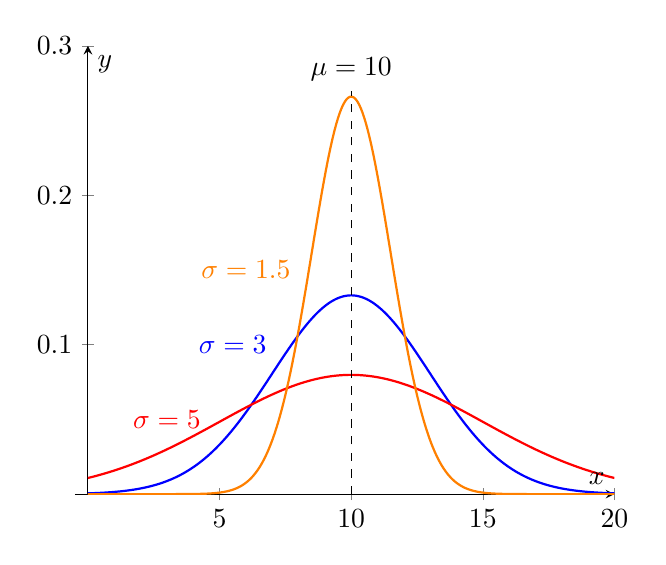
\begin{tikzpicture}
	\begin{axis}[xmin = -0.5, xmax = 20, ymin = 0, ymax = 0.3, axis lines = 
	center, xlabel = $x$, ylabel = $y$]
		\addplot[blue, thick, domain = 0:20, samples = 300] 
		{1/(3*sqrt(2*3.14159))*e^(-(x - 10)^2/(2*3^2))};
            \addplot[red, thick, domain = 0:20, samples = 300] 
            {1/(5*sqrt(2*3.14159))*e^(-(x - 10)^2/(2*5^2))};
            \addplot[orange, thick, domain = 0:20, samples = 300] 
            {1/(1.5*sqrt(2*3.14159))*e^(-(x - 10)^2/(2*1.5^2))};
            \node[orange] at (6, 0.15) {$\sigma = 1.5$};
            \node[blue] at (5.5, 0.1) {$\sigma = 3$};
            \node[red] at (3, 0.05) {$\sigma = 5$};
            \draw[black, dashed] (10, 0) -- (10, 0.27) node[above] {$\mu = 10$};
		\end{axis}
	\end{tikzpicture}
    \label{fig:stddevs}
    \caption{Changing $\sigma$ affects the width of the distribution, but not 
    its center}
\end{figure}

\textbf{Example}: Birth weights in the United States are normally distributed 
with a mean of 7 lbs 6 oz and a standard deviation 1 lb 2 oz. Write a PDF to 
represent this data. What percentage of US babies are born at less than 5 lbs? 
Over 9 lbs?

\textbf{Solution}: For simplicity, let us express everything in ounces. Recall 
that there are 16 oz in a pound. Therefore, 
$$\mu = 118\text{ oz}$$
$$\sigma = 18\text{ oz}$$

And we can write the PDF for US birth weight:
$$f(x) = \frac{1}{18\sqrt{2\pi}}e^{-\left(x - 118 \right)^2/\left(2 \left( 18 
\right)^2 \right)}$$

To find the percentage of babies with a birth weight below 5 lbs, we integrate 
from 0 (since a baby must have some weight) to 80 oz (the equivalent of 5 lbs):
$$P(X \leq 80) = \int_0^{80} \frac{1}{18\sqrt{2\pi}}e^{-\left(x - 118 \right)^2/
\left(2 \left( 18 \right)^2 \right)}\,dx$$

Unfortunately for us, there is no anti-derivative to $e^{-x^2}$, so we cannot 
evaluate the integral by hand. However, you can use a calculator or computer 
to find the approximate value of the integral. Inputting the integral into a 
calculator (such as a TI-89), we find that:
$$P(X \leq 80) \approx 0.0174$$

And therefore, approximately 1.74\% of US babies are born weighing less than 5 
lbs. 

To find the percentage of babies born weighing more than 9 lbs, we integrate 
from 144 oz to infinity (obviously, babies are not born with infinite weight, 
but this will do just fine for an approximation):
$$P(X \geq 144) = \int_{144}^{\infty} \frac{1}{18\sqrt{2\pi}}e^{-\left(x - 118 
\right)^2/\left(2 \left( 18 \right)^2 \right)}\,dx$$

Again, using a calculator or computer, we find that:
$$P(X \geq 144) \approx 0.0743$$

And therefore approximately 7.43\% of US babies are born weighing more than 9 
lbs.
